%___________________________________________
% 4) Função recíproca f(x) = 1/x
%___________________________________________
\begin{figure}[H]
  \centering
  \begin{tikzpicture}
    \begin{axis}[
      xmin=-4, xmax=4,
      ymin=-4, ymax=4,
      axis x line=middle,
      axis y line=middle,
      axis line style={-},
      tick align=outside,
      grid=both,
      minor tick num=1,
      xlabel={$x$},
      ylabel={$y$},
      title={$f(x)=\dfrac{1}{x}$}
    ]
      % ramos esquerda e direita (evitando x=0)
      \addplot[red, domain=-4:-0.05, samples=200] {1/x};
      \addplot[blue, domain=0.05:4, samples=200] {1/x};
    \end{axis}
  \end{tikzpicture}
  \caption{Função recíproca $f(x)=1/x$.}
\end{figure}